\documentclass[runningheads]{llncs}
%
\usepackage[T1]{fontenc}
%
\usepackage{graphicx}
%

% Daniel Motz's packages
\usepackage{amsfonts}
\usepackage{amsmath}
\usepackage{stmaryrd}
\usepackage{amssymb}
\usepackage{mathtools}
\usepackage{ bbold }
\DeclarePairedDelimiter\ceil{\lceil}{\rceil}
\DeclarePairedDelimiter\floor{\lfloor}{\rfloor}

\usepackage{tikz}
\usepackage{tikz-3dplot}
\usepackage{pgfplots}
\pgfplotsset{compat = newest}

\usepackage{hyperref}

\usepackage{setspace}
\doublespacing

\renewcommand{\abstractname}{}
\newcommand{\inline}{\mintinline[fontsize=\normalsize]{c++}{text}}
\DeclareUnicodeCharacter{03BB}{$\lambda$}
% END Daniel Motz's packages

\begin{document}
%
\title{
    Automaten und Berechenbarkeit
}
%
\titlerunning{A\&B}%
\author{Maximilian Stock, Daniel Motz}
%
\authorrunning{M. Stock, D. Motz}
%
\institute{Fakultät für Mathematik und Informatik, Friedrich-Schiller-University,\\ Jena, Germany\\
\vspace{.2cm}
\email{maximilian.stock@uni-jena.de, daniel.motz@uni-jena.de}
}
%
\maketitle % typeset the header of the contribution
%

\section{Endliche Automaten und reguläre Sprachen}

\subsection{Alphabete, Wörter und Sprachen}

Die Darstellung von Daten -- als Eingabe für Algorithmen -- wird realisiert als "Wörter".

\begin{example}
    Darstellung von Graphen

    \begin{minipage}{0.5\linewidth}
        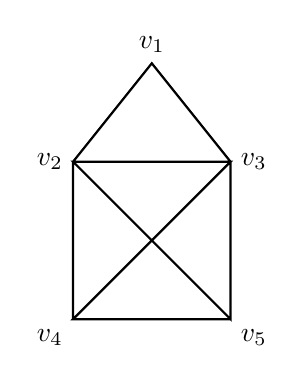
\begin{tikzpicture}[domain=0:4]
            \draw[thick,sharp corners=0pt]
            (0,0) node[anchor=north east]{$v_4$} --
            (0,2) node[anchor=east]{$v_2$} -- 
            (1,3.25) node[anchor=south]{$v_1$} --
            (2,2) node[anchor=west]{$v_3$} -- 
            (2,0) node[anchor=north west]{$v_5$} -- 
            (0,2) --
            (2,2) -- 
            (0,0) -- 
            (2,0);
        \end{tikzpicture}
    \end{minipage}
    
    \begin{minipage}{0.5\linewidth}
        $\begin{matrix}
            & v_1 & v_2 & v_3 & v_4 & v_5 \\
        v_1 & 0 & 1 & 1 & 0 & 0 \\
        v_2 & 1 & 0 & 1 & 1 & 1 \\
        v_3 & 1 & 1 & 0 & 1 & 1 \\
        v_4 & 0 & 1 & 1 & 0 & 1 \\
        v_5 & 0 & 1 & 1 & 1 & 0
        \end{matrix}$
    \end{minipage}
\end{example}

\end{document}
